\section{Introduction}

\section{Experimental Design}
Overview

\subsection{Participant Recruitment and Incentives}
Participants will be recruited to discuss a policy issue
using a custom-built psudeonymous online platform.
The policy issue will be chosen to be relevant to many individuals,
and to be amenable to a predefined list of proposed solutions,
as well as to be relevant at the time the experiment is conducted.
Example policy questions include
``Where should the use of electric scooters be permitted?'' and
``Given the COVID-19 pandemic, how should schools in the US reopen in Fall 2021?.''
Multiple waves of deliberation may be held using different questions and participants,
depending factors such as participant attrition.

Participants will be recruited using a number of methods.
Participants will be recruited individually through posts on web forums
relevant to the policy question (e.g., reddit),
relevant facebook groups,
and relevant email lists.
Participant pools will also be utilized,
such as lists of previous participants who have expressed interest in future
studies,
and the UMSI Online Recruitment System for Economic Experiments.
Individual participants will also be recruited using promoted posts and
advertisements on Twitter, Facebook, etc.
Separately, participants may also be recruited through partnership with
community groups who wish to try network deliberation as part of an organizational
decision-making strategy.
The number of such collaborations will depend on the number of sufficiently-large
partner organizations that have decisions amenable to network deliberation
over the course of the experiment.

All participants will be paid incentives for participation in the deliberation
and completion of ranked-choice votes and pre/post-experiment surveys.
It is crucial that the incentive structure incentivize participation,
without incentivizing any particular deliberative strategy
(e.g., prefering a specific outcome, maintaining an original position, or
seeking agreement/disagreement).
Any such incentive structure could motivate participants to act based on their
preferences for incentive payments rather than their true preferences regarding
the policy question under consideration,
and disincentivize honest deliberation about the policy question.
As such, incentives will be paid as the same fixed amount to all participants.

The minimum number of participants required is determined by a number of factors.
First, the long-path pod assignment method results in a minimum number of pods,
determined by the chosen parameters.
Specifically, the pod assignments for each round beyond the first are determined
by a unique prime number,
and the number of pods is a multiple of that prime.
For $T=3$ rounds, two primes are necessary and choosing the lowest two (2, 3)
yields the lowest minimum number of pods: 3.
For all pods to have at least 4 members, the minimum number of participants in
the long-path treatment is 12.

The two network deliberation treatments must also have meaningfully different
structural properties,
which also necessitates a minimum number of participants.
Structural differences between these two networks become more pronounced
with a greater number of participants.
While properties such as the broadcast time (see Chapter \ref{chap:abm})
and average geodesic length can be used to compare the structural efficiency of
two networks,
they encounter a problem for these particular networks
when there is a small number of rounds:
for many pairs of individuals, no path will exist.
In practical terms,
an idea proposed by one participant may not have a plausible
path to reach some of the other participants by the end of the deliberation,
even if that idea is repeatedly shared by all who encounter it.
As an alternative, a form of k-connectivty can be used to measure
structural efficiency.
The k-connectivity is simply the fraction of possible paths that exist.
In other words, if each participant broadcasts a message, and that message is
repeated by all who encounter it, what is the average fraction of participants
a broadcast will reach?
Figure \ref{fig:kcon} shows the k-connectivity as a function of number of
participants for both the long-path and random-pod deliberation networks.
While there is no clear threshold for the necessary number of participants,
choosing a k-connectivity of $0.5$ (half of possible paths exist) seems a
reasonable heuristic.
For the chosen parameters, 35 or more participants are necessary to produce
a random-pod network with $>0.5$ k-connectivity and
a long-path network with $<0.5$ k-connectivity.

Combining the above considerations,
an absolute minimum of 12 participants per treatment is necessary to conduct
a wave of the experiment,
and a minimum of about 35 participants per treatment group is necessary to
observe differences between the network deliberation treatment conditions.

\begin{figure}
\label{fig:kcon}
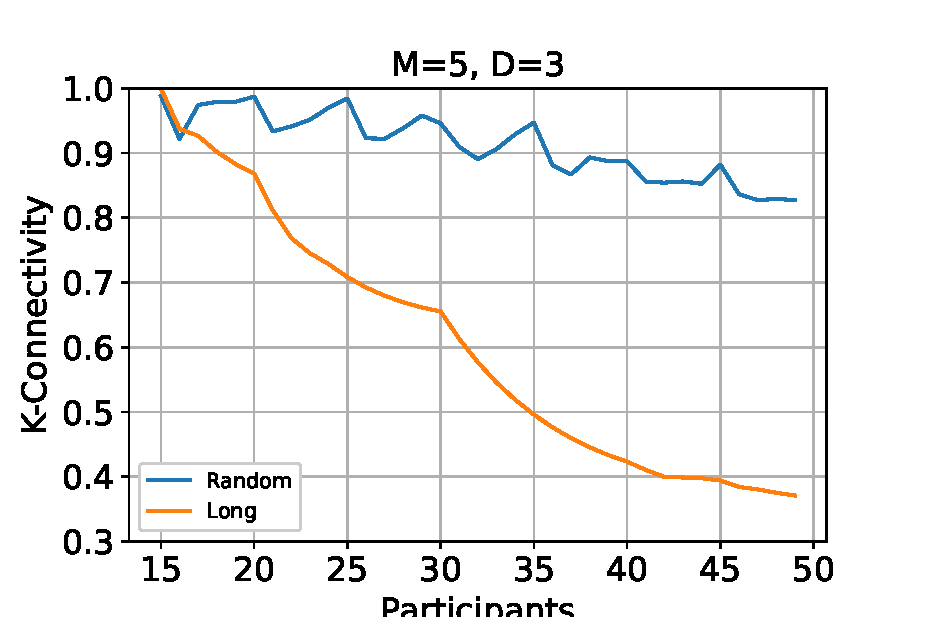
\includegraphics[width=5in]{fig/Experiment/fig-kcon.eps}
\caption{The k-connectivity of long-path and random-pod network deliberation
networks for $T=3$ stages and a pod size of $M=5$.}
\end{figure}

\subsection{Experimental Protocol}

At the beginning of the experiment, participants will complete a short
demographic survey.
This survey will enable the identification of sample bias in age, gender, race,
and other demographic factors.

When participants are enrolled, they will be assigned to one of three treatment
groups: control, random-pod, long-path.
The control group will deliberate in a single large group.
The random-pod and long-path treatments will deliberate in a series of small
pods (network deliberation).
These treatments will vary only by the pod assignment method used:
either random-pod or long-path (see Chapter \ref{chap:abm}).

Deliberation will be divided into a predetermined number of {\em rounds}, each lasting
a fixed length of time.
Current plans are to use three stages of two days each,
although these numbers may need to be changed
to ensure time timeline of the deliberation is consistent with any constraints
imposed by specific policy questions.
Before and after each stage, participants will be asked to rank the proposed
solutions to the policy question according to their individual preference.
During each round, participants will be shown a discussion prompt and will be
able to post and reply to other participants.
Example prompts are shown in Table \ref{tab:prompts}.
Participants will only be able to see or interact with posts from others in
their current pod.
(all control group participants will be able to interact with all others
at all times).
Participants will be able to view posts and comments that were visible to them
in previous rounds, but will no longer be able to interact with or reply to
those posts and comments.

\begin{table}
\center
\label{tab:prompts}
\begin{tabular}{|p{0.3in}|p{3.6in}|}
\hline
Stage & Prompt \\
\hline
1 &
Which proposals do you prefer, and why?
If there are disagreements, try asking questions to understand the perspective
of others and to understand the causes of the disagreement.
\\
\hline
2 & In the previous round of discussion, what opinions and reasoning did you
observe in your group?
How much agreement was there?
Were there any disagreements or conflicts?
If so, what were the sources of conflict, and how might they be resolved?
\\
\hline
3 &
What seem to be the most popular opinions?
Do you agree with them?
Has your opinion changed over the course of the discussion?
\\
\hline
\end{tabular}
\end{table}

A subset of participants will be randomly selected to participate in
60-minute semi-structured interviews about their experience.
These interviewed will be qualitatively coded using grounded theory.
The interviews will provide information on the subjective experience of
participants, as well as help identify common themes that may provide
insight into the strengths and weaknesses of network deliberation.

In summary, the experiment will result in several data sets:
\begin{itemize}
\item The ranked choice preferences of each participant before and after each round of deliberation.
\item The text of the online deliberation.
\item Post-deliberation survey responses.
\item Qualitatively-coded interview transcripts.
\end{itemize}

\subsection{Quantifying Preferences, Conflict, and Agreement}

\section{Study Software}

\section{Pilot Studies}
Several pilot studies have already been conducted:
one in a synchronous lab setting, and two using the asynchronous online
software.
In addition to providing an opportunity to test software,
these pilot studies have provided crucial information for developing a
feasible experimental design.

The initial pilot study was conducted on December 21, 2018,
before the custom online platform was developed.
In this pilot, NUMBER participants engaged in a synchronous 60-minute deliberation.
Participants sat at individual computer workstations, separated by dividers.
Participants discussed the following question:
``Where should the use of electric scooters be permitted?''
Participants were placed in a single treatment group, and divided into 4
pods of size 4--5.
These pods were reassigned using the random-pod method for a total of three
rounds.
The deliberation took place in chat rooms running the free and open-source
OTree online experiment software.

The second pilot took place after the initial development of the custom online
platform, from August 24, 2020 through August 32, 2020.

The third pilot took place from August 23, 2021 through August 29, 2021.

